\documentclass[a4paper]{article}

%% Language and font encodings
\usepackage[english]{babel}
\usepackage[T1]{fontenc}

%% Sets page size and margins
\usepackage[a4paper,top=3cm,bottom=2cm,left=3cm,right=3cm,marginparwidth=1.75cm]{geometry}

% Useful packages
\usepackage{amsmath}
\usepackage{graphicx}
% \usepackage[colorinlistoftodos]{todonotes}
\usepackage[colorlinks=true, allcolors=blue]{hyperref}

\title{COP290 C LAB: SPREADSHEET PROGRAM}
\author{Samarth Patel, Priyanka Sar, Rishika Garg}

\begin{document}
\maketitle

\begin{abstract}
Your abstract.
\end{abstract}

\section{DESIGN DECISIONS}

Our spreadsheet program consists of a Makefile that compiles our source files: \texttt{asscop.c}, \texttt{display.c}, \texttt{expcalc.c}, \texttt{graph.c}, \texttt{avltree.c}, and \texttt{helper.c} to create an executable spreadsheet-like application. This spreadsheet accepts formulas and control inputs.

\texttt{Display.c} initializes our sheet with the required number of rows and columns, with each cell initialized to zero. Upon receiving input, it calls the \texttt{getline} function (defined in \texttt{helper.c}) to read commands, scroll the sheet, or disable/enable the display. If necessary, it invokes the parser (defined in \texttt{asscop.c}) for assignments, recalculations or to raise errors when the command is invalid. 

Each cell in our spreadsheet is a structure containing:
\begin{itemize}
    \item Its current value,
    \item Values of sums and square sums for easy recalculations (\texttt{sum} variable is also used for keeping the new value after updating),
    \item A visit marker for graph traversal,
    \item Value of rows and columns on which it is dependent (for range we just store the two end points),
    \item Its error count (count of error-prone cells on which it is dependent),
    \item A \texttt{count} variable that denotes the number of cells on which it is dependent among all the nodes in the graph (of affected cells),
    \item Pointers to AVL tree roots for dependency tracking and min/max calculations.
\end{itemize}

We utilize AVL trees (\texttt{avltree.c}) to efficiently manage dependencies and perform operations such as \texttt{MIN} and \texttt{MAX} in logarithmic time. Additionally, the spreadsheet maintains a directed graph, where each cell is represented as a node. A directed edge from cell $A$ to cell $B$ indicates that $B$ depends on $A$. This structure enables efficient propagation of updates, ensuring that only affected dependent cells are recalculated when a modification occurs.

To further optimize updates, we implement a deferred update mechanism. When a cell is modified, both its old and new values are stored. Instead of immediately propagating the new value to dependent cells, we first process all necessary recalculations while maintaining the old values. Once all affected cells have been updated, a final commit operation is executed to store the new values. This approach minimizes redundant computations and enhances overall efficiency.

\section{EDGE CASES AND ERROR SCENARIOS}

\subsection{Padding for 32-bit Integers}
We added a padding of 15 in \texttt{display.c} to ensure that signed 32-bit integers are displayed correctly.

\subsection{Invalid Range}
Providing invalid ranges in functions such as MAX, MIN, SUM, AVG, and STDEV results in an error. Examples:
\begin{enumerate}
    \item \texttt{A1=AVG(B2:B1)} will output: \textbf{[0.0] (invalid range) >}
    \item \texttt{A1=SUM(A100:F1)} will output: \textbf{[0.0] (invalid range) >}
\end{enumerate}

\subsection{Invalid Commands}
Various invalid input commands are handled:
\begin{enumerate}
    \item Empty range functions such as \texttt{SLEEP()}, \texttt{MAX()}, \texttt{MIN()}, \texttt{AVG()}, \texttt{SUM()} all return \textbf{[0.0] (unrecognized cmd) >}
    \item Missing parentheses or incorrect syntax in functions, e.g., \texttt{A1=MAX(B1:B2}, \texttt{A1=MAX(B1 B2)}, \texttt{A1=MAX B1:B2)}, return \textbf{[0.0] (unrecognized cmd) >}
    \item Other invalid inputs can also be like
    \textttA{A4=AVG(A1:A3)xyz}, \texttt{A1=MAX(B1 B2)}, \texttt{A4=A5MIN(A3:A3)}, return \textbf{[0.0] (unrecognized cmd) >}
\end{enumerate}

\subsection{Cyclic Dependency}
If a formula creates a cyclic dependency (e.g., \texttt{A1=B1+1} and \texttt{B1=A1+1} or \texttt{A10=MAX(A5:A10)}), our program detects this and prevents infinite loops. The output will be:
\begin{center}
    \textbf{[0.0] (cycle detected) >}
\end{center}

\subsection{Division by Zero}
Any division by zero, such as \texttt{A1=B1/0}, results in an error. The cell value will be:
\begin{center}
    \textbf{ERR}
\end{center}
The program ensures that cell is assigned ERR till it is reassigned correctly instead of halting the program.

\subsection{Invalid Cells}
Accessing non-existent cells results in an error. For example:
\begin{enumerate}
    \item \texttt{A1=B10000+5} (when the sheet has only 100 rows)
    \item \texttt{X1=SUM(A1:A2)} (when column X does not exist)
    \item \texttt{scrollto ZZZ1000} 
\end{enumerate}
Such cases return:
\begin{center}
    \textbf{[0.0] (invalid cell) >}
\end{center}

\subsection{Incorrectly Running the Program}
Running the program with noninteger or out of range integer inputs in the row and column (e.g.nge (e.g. \texttt{./sheet six forty}) will result in:
\begin{center}
    \textbf{error: write valid number of rows and columns.}
\end{center}

\begin{figure}
\centering
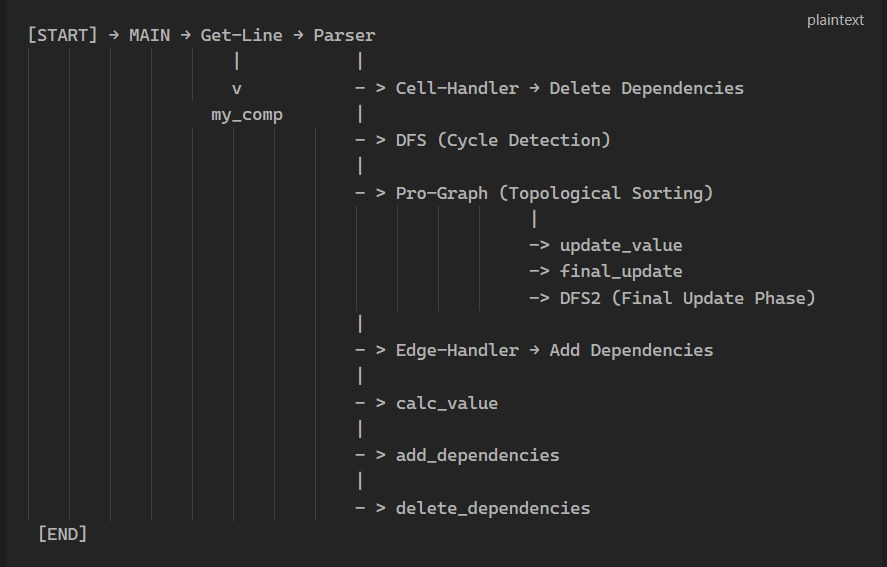
\includegraphics[width=0.3\textwidth]{copass.jpg}
\caption{Example output of the spreadsheet program.}
\end{figure}

\section{STRUCTURE OF PROGRAM}

\begin{enumerate}
    \item Display.c
    \begin{itemize}
        \item int main(int argc, char *argv[])
        \item void display (cell ** mysheet, int R, int C, int x, int y)
        \item char * print\_string(int n, int padding)
    \end{itemize}
    \item Asscop.c:
    \begin{itemize}
        \item char parser(char* input)
        \item bool edgehandler (int cellhandle, int lhs, cell* lhscell, int extra, cell oldcell)
        \item void addDependencies (cell * lhscell, char op, int lhs)
        \item void deleteDependencies(cell *lhscell, int lhs)
        \item int cell\_handler(char *cell)
        \item bool is\_int (char *s)
    \end{itemize}
\end{enumerate}


\section{How to Add Lists}
Lists can be created using:
\begin{enumerate}
    \item Automatic numbering:
    \begin{enumerate}
        \item Like this,
        \item And like this.
    \end{enumerate}
    \item Bullet points:
    \begin{itemize}
        \item Like this,
        \item And like this.
    \end{itemize}
\end{enumerate}

\end{document}
